\documentclass[a4paper]{article}
% Uncomment the following line to allow the usage of graphics (.png, .jpg)
\usepackage{graphicx}
% Allow the usage of utf8 characters
\usepackage[utf8]{inputenc}
\usepackage{enumerate}
\usepackage{amssymb}
\usepackage{colortbl}
\usepackage{icomma}
\usepackage{booktabs}
\usepackage{siunitx}
\sisetup{locale=DE}
\usepackage{tikz}
\usepackage{href-ul}
\hypersetup{
	colorlinks=true,
	linkcolor=blue,
	urlcolor=blue}
\usepackage{geometry}
\geometry{a4paper, top=15mm, left=15mm, right=15mm, bottom=15mm,
	headsep=10mm, footskip=12mm}

\begin{document}
	
	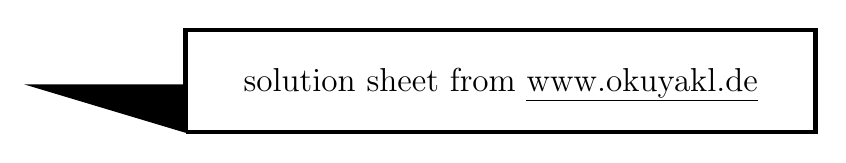
\begin{tikzpicture}(10,3)
		\draw[ultra thick](2,0) --(10,0) -- (10,1.3) --(2,1.3) -- (2,0);
		\draw[fill=black](2,0)-- (0,.6) -- (2,.6) -- (2,0);
		\node at (6,.6) {\large solution sheet from \href{https://www.okuyakl.de}{www.okuyakl.de}};
	\end{tikzpicture}
	
	
	\section*{1. The Lazy Cat and the Hot Water Bottle}
		
		\begin{itemize}
			\item \( m = 2\,\text{kg} \) (2 L water),
			\( \Delta \vartheta = 60^\circ C - 20^\circ C = 40\,\text{K} \),
			\( c = 4{,}18\,\frac{\text{kJ}}{\text{kg}\cdot\text{K}} = 4180\,\frac{\text{J}}{\text{kg}\cdot\text{K}} \)
			
			\item a)
			\[
			Q = 4180 \cdot 2 \cdot 40 = \underline{334400\,\text{J}}\approx 0.33 \,\text{MJ}
			\] 
			
			\item b) \( Q_\text{heat} = 80\,\% \) of 334400 J:
			\[
			Q = 0.8 \cdot 334.400 = \underline{267520\,\text{J}}\approx 0.27 \,\text{MJ}
			\]
		\end{itemize}
		
		\hrulefill
		
		\section*{2. The Spaghetti Action}
		
		\begin{itemize}
			\item \( m = 0.5\,\text{kg} \),
			\( \Delta \vartheta = 100^\circ C - 15^\circ C = 85\,\text{K} \)
			
			\item a)
			\[
			Q = 4180 \cdot 0.5 \cdot 85 = \underline{177650\,\text{J}}\approx 0.18\, \text{MJ}
			\]
			
			\item b) Actual energy consumption at 80 \% efficiency:
			\[
			Q = \frac{177650}{0.8} = \underline{222063\,\text{J}}\approx 0.22 \,\text{MJ}
			\]
		\end{itemize}
		
		\hrulefill
		
		\section*{3. The bathtub for astronauts}
		
		\begin{itemize}
			\item \( m = 100\,\text{kg} \),
			\( \Delta \vartheta = 20\,\text{K} \)
			
			\item a)
			\[
			Q = 4180 \cdot 100 \cdot 20 = \underline{8360000\,\text{J}}\approx 8.4\, \text{MJ}
			\]
			
			\item b) Duration: 10 minutes = 600 seconds.
			Each heating element (1000 W) produces 600,000 J in 10 minutes.
			\[
			\frac{8360000}{600000} = \underline{13{,}93 \approx 14 \,\text{ heating elements}}
			\]
		\end{itemize}
		
		\hrulefill
		
		\section*{4. The lukewarm declaration of love}
		
		\begin{itemize}
			\item \( m = 0.25\,\text{kg} \),
			\( \Delta \vartheta = 35\,\text{K} \)
			
			\item a)
			\[
			Q = 4180 \cdot 0.25 \cdot 35 = \underline{36575\,\text{J}}\approx 37 \,\text{kJ}
			\]
			\item b) With a 10 \% loss $\Rightarrow$ 90 \% = \( 0.9 \cdot Q_\text{real} = 36575\,\text{J} \)
			\[
			Q_\text{real} = \frac{36575}{0{,}9} = \underline{40639\,\text{J}}\approx 41 \,\text{kJ}
			\]
		\end{itemize}
		
		
		\section*{5. The hot screw }
		
		\begin{itemize}
			\item a) \( m = 0{.}3\,\mathrm{kg} \), \( \Delta \vartheta = 160\,\mathrm{K} \), \( c = 450 \,\frac{\mathrm{J}}{\mathrm{kg}\cdot\mathrm{K}}\)
			
			\[
			Q = 450 \cdot 0{.}3 \cdot 160 = \underline{21600\,\text{J}}\approx 22 \,\text{kJ}
			\]
			
			\item b) \( m = 0{.}6\,\text{kg} \)
			
			\[
			Q = 450 \cdot 0{.}6 \cdot 160 = \underline{43200\,\text{J}}\approx 43\, \text{kJ}
			\]
		\end{itemize}
		
		\hrulefill
		
		\section*{6. The melting butter }
		
		\begin{itemize}
			\item a) \( m = 0{.}25\,\mathrm{kg} \), \( \Delta \vartheta = 34\,\mathrm{K} \), \( c = 2100 \,\frac{\mathrm{J}}{\mathrm{kg}\cdot\mathrm{K}}\)
			
			\[
			Q = 2100 \cdot 0{.}25 \cdot 34 = \underline{17850\,\text{J}}\approx 18 \,\text{kJ}
			\]
			
			\item b) \( Q = 17{.}850\,\mathrm{J} \), \( m = 0{.}125\,\mathrm{kg} \)
			
			\[
			\Delta \vartheta = \frac{Q}{c \cdot m} = \frac{17{.}850}{2100 \cdot 0{.}125} = \underline{68\,\text{K}}
			\]
		\end{itemize}
		
		\hrulefill
		
		\section*{7. The Fiery Brick }
		
		\begin{itemize}
			\item \( m = 2\,\text{kg} \), \( \Delta \vartheta = 875\,\text{K} \), \( c = 840\,\frac{\text{J}}{\text{kg}\cdot\text{K}} \)
			
			\[
			Q = 840 \cdot 2 \cdot 875 = \underline{1470000\,\text{J}}\approx 1.5 \,\text{MJ}
			\]
			
			\item b) The color influences the absorption of thermal radiation: dark colors like red or black absorb more radiation → faster heating.
		\end{itemize}
		
		\hrulefill
		
		\section*{8. The cheese cube in the toaster }
		
		\begin{itemize}
			\item \( m = 0{.}05\,\mathrm{kg} \), \( \Delta \vartheta = 50\,\mathrm{K} \), \( c = 3100 \,\frac{\mathrm{J}}{\mathrm{kg}\cdot\mathrm{K}}\)
			
			\[
			Q = 3100 \cdot 0{.}05 \cdot 50 = \underline{7750\,\text{J}}
			\]
			
			\item \( P = 150\,\text{W} \), so \( t = \frac{Q}{P} = \frac{7750}{150} \approx \underline{52\,\text{s}} \)
		\end{itemize}
		
		\hrulefill
		
		\section*{9. Sauna with wooden bench }
		
		\begin{itemize}
			\item a) \( m = 1{.}5\,\mathrm{kg} \), \( \Delta \vartheta = 50\,\mathrm{K} \), \( c = 1700\,\frac{\mathrm{J}}{\mathrm{kg}\cdot\mathrm{K}} \)
			
			\[
			Q = 1700 \cdot 1{.}5 \cdot 50 = \underline{127500\,\text{J}}\approx 0.13 \,\text{MJ}
			\]
			
			\item b) \( c_\text{Alu} = 900 \)
			
			\[
			Q = 900 \cdot 1{.}5 \cdot 50 = \underline{67500\,\text{J}}\approx 68\,\text{kJ}
			\]
		\end{itemize}
		
		
	\begin{center}
		\includegraphics[width=7 cm]{../../viecher/eendcomic.pdf}
		
		Click here to return to the \href{https://www.okuyakl.de/phys/p9qcmL116/ae116.pdf}{worksheet}
	\end{center}
	\end{document}